\documentclass{article}
\usepackage{xeCJK,amsmath,geometry,graphicx,amssymb,zhnumber,booktabs,setspace,tasks,verbatim,amsthm,amsfonts,mathdots}
\usepackage{listings,xcolor,float,caption,subfigure}
\geometry{a4paper,scale=0.8}   
\title{ICS  HomeWork-2}
\author{PB20000113孔浩宇}
\begin{document}
\maketitle
\section*{T1}
    \begin{enumerate}
        \item [(a)]$S=0,\ E=1,\ M=0\ (normalized)$
        \begin{align*}
            Min
            &=0\ 0000 0001\  000\ 0000\ 0000\ 0000\ 0000\ 0000\\
            &={(-1)}^{S}\times 1.M\times 2^{E-127}\\
            &=2^{-126}.
        \end{align*}
        \item [(b)]$S=0,\ E=0,\ M=111\ 1111\ 1111\ 1111\ 1111\ 1111,\ (subnormal)$
        \begin{align*}
            Max
            &=0\ 0000 0000\ 111\ 1111\ 1111\ 1111\ 1111\ 1111\\
            &={(-1)}^{S}\times 0.M \times 2^{-126}\\
            &=1.1111111111111111111111\times 2^{-127}.
        \end{align*}
    \end{enumerate}

\section*{T2}
\begin{align*}
    Max
    &={(0111\ 1111\ 1111\ 1111\ 1111\ 1111\ 1111\ 1111)}_{\mbox{补}}\\
    &={(0111\ 1111\ 1111\ 1111\ 1111\ 1111\ 1111\ 1111)}_{\mbox{原}}\\
    &=2^{31}-1.
\end{align*}
\section*{T3}如图$1$.
\begin{figure}
    \centering
    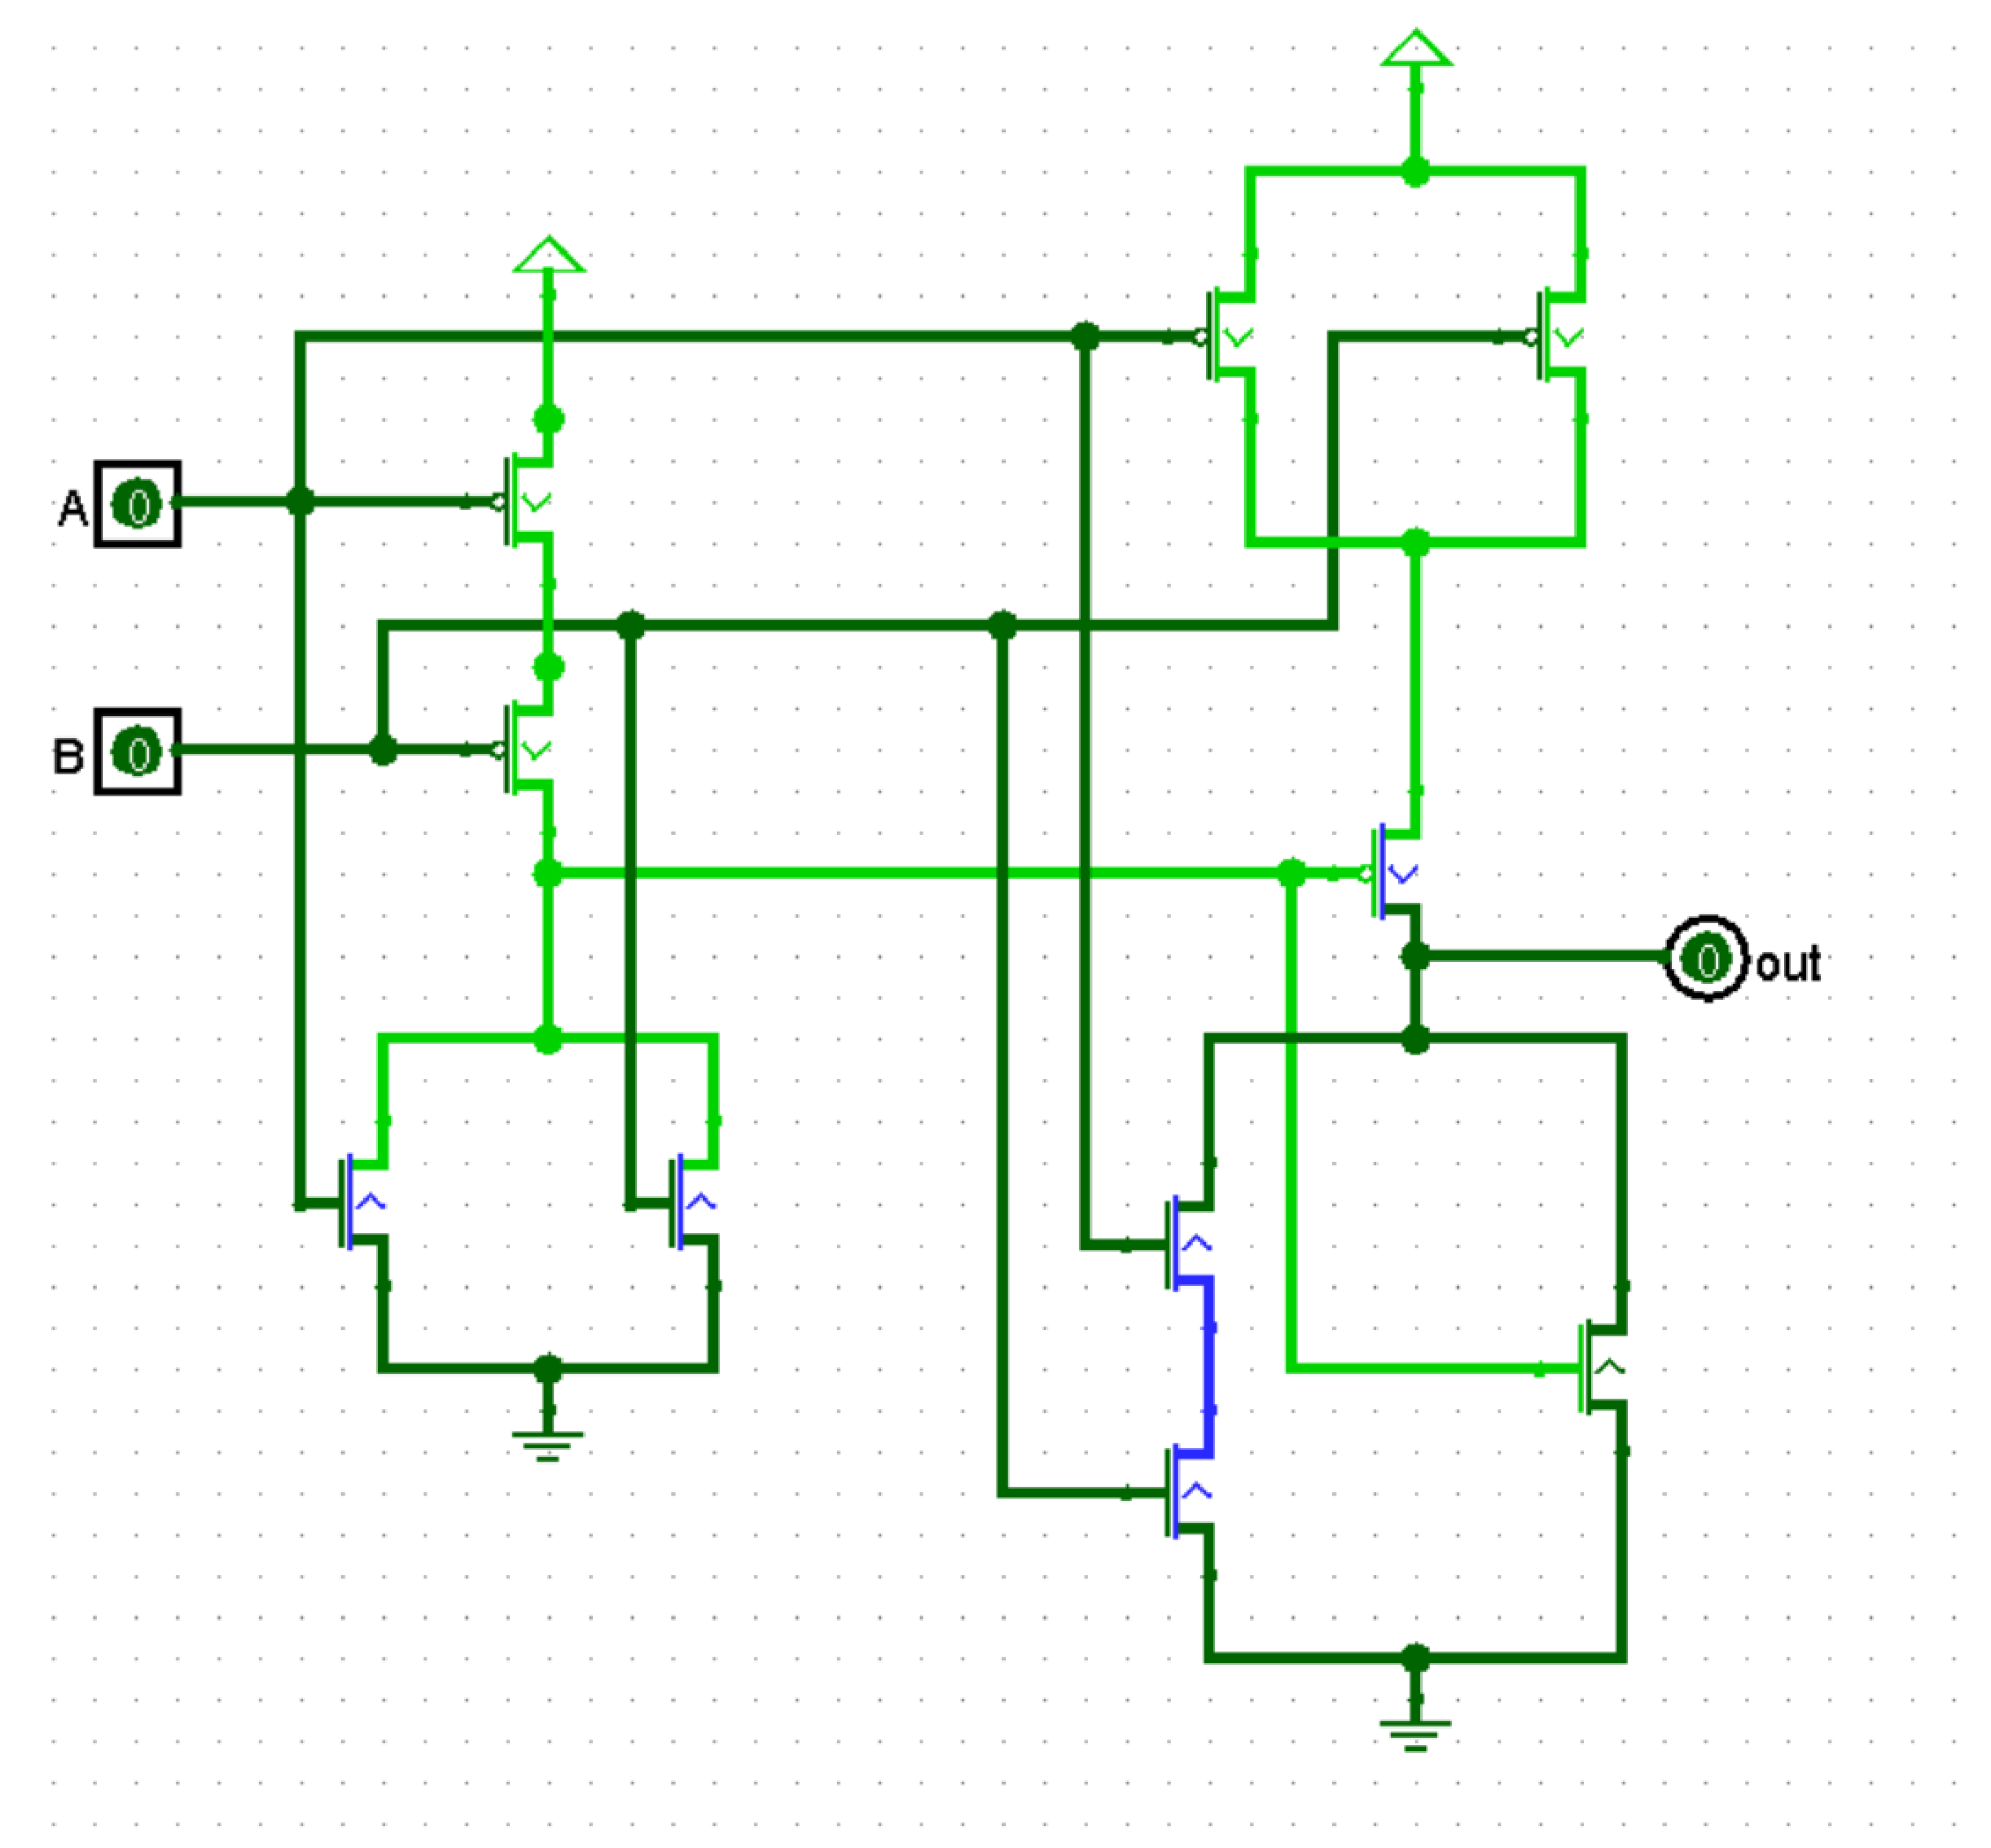
\includegraphics[scale=0.3]{picture/xor.eps}
    \caption{T3}
\end{figure}
\section*{T4}$A,B,C$分布如图$2$所示。两种情况真值表相同,如下。
\begin{table}[!ht]
    \centering
    \begin{tabular}{|c|c|c|c|}
    \hline
        A & B & C & out  \\ \hline
        0 & 0 & 0 & 1  \\ \hline
        0 & 0 & 1 & 1  \\ \hline
        0 & 1 & 0 & 1  \\ \hline
        0 & 1 & 1 & 1  \\ \hline
        1 & 0 & 0 & 1  \\ \hline
        1 & 0 & 1 & 0  \\ \hline
        1 & 1 & 0 & 0  \\ \hline
        1 & 1 & 1 & 0  \\ \hline
    \end{tabular}
\end{table}
\begin{figure}[htbp]
    \centering
    \subfigure[]
    {
        \begin{minipage}{7cm}
            \centering
            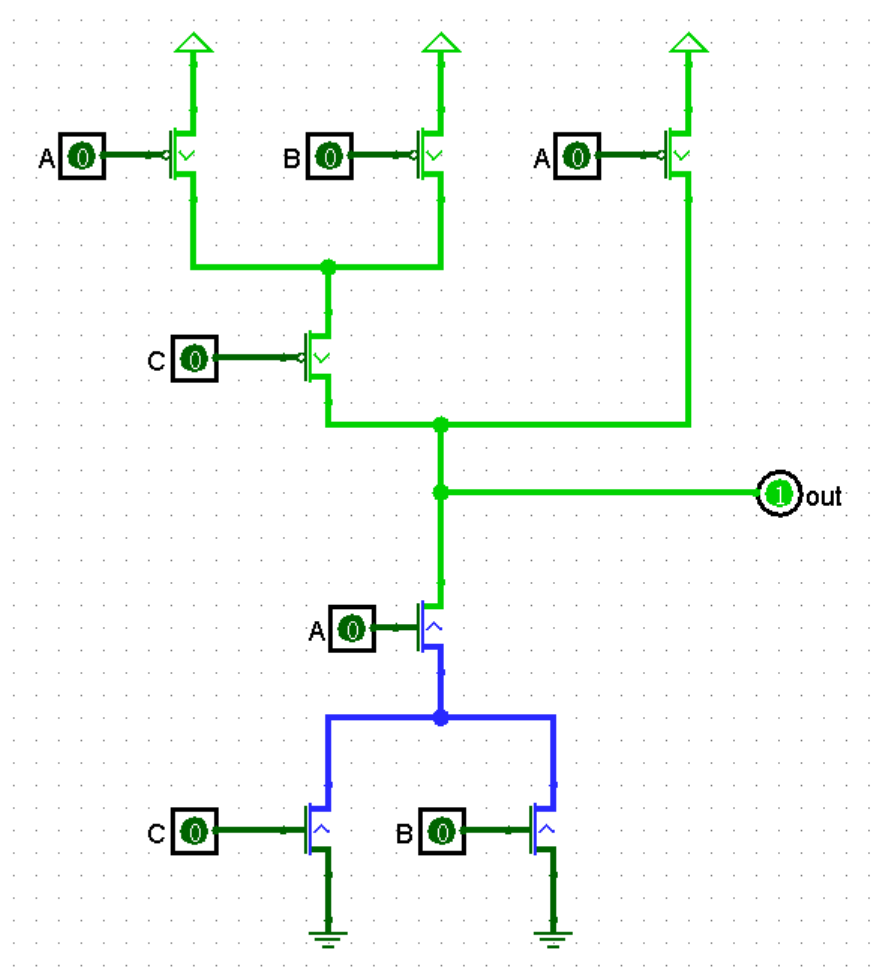
\includegraphics[scale=0.45]{picture/T41.png}
        \end{minipage}
    }
    \subfigure[]
    {
        \begin{minipage}{7cm}
            \centering
            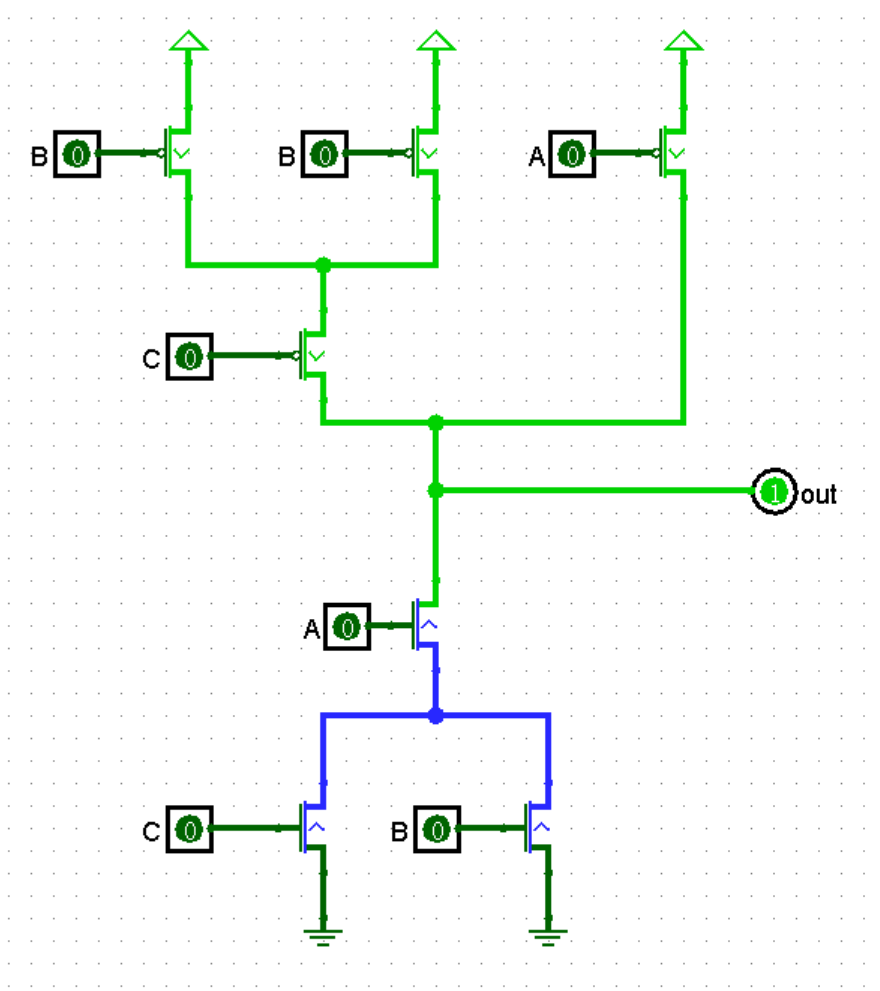
\includegraphics[scale=0.45]{picture/T42.png}
        \end{minipage}
    }
    \caption{T4}
\end{figure}
\clearpage

\section*{T5}
\begin{align*}
    0\ \mbox{OR}\ X& = X;\\
    1\ \mbox{OR}\ X& = 1;\\
    0\ \mbox{AND}\ X& = 0;\\
    1\ \mbox{AND}\ X& = 1;\\
    0\ \mbox{XOR}\ X& = X.
\end{align*}

\section*{T6}
    \begin{enumerate}
        \item [(1)]当$A=0$时,$D$与$C$保持一致;当$A=1$时,$D$与$B$保持一致。
        \item [(2)]当$(A,B)$转变到$(1,1)$时,$D$保持不变;当$(A,B)$转变到$(1,0)$时,$D$变为$0$;
        当$(A,B)$转变到$(0,1)$时,$D$变为$1$;当$(A,B)$转变到$(0,0)$时,$D$的状态不能确定。
    \end{enumerate}
\section*{T7}
    \begin{enumerate}
        \item [(a)]有32bits输出。
        \item [(b)]1bit output. 4bits select.
    \end{enumerate}

\section*{T8}
    \begin{enumerate}
        \item [1.]3. (S到达输出有3个门延迟)
        \item [2.]如图.
        \begin{figure*}[htbp]
            \centering
            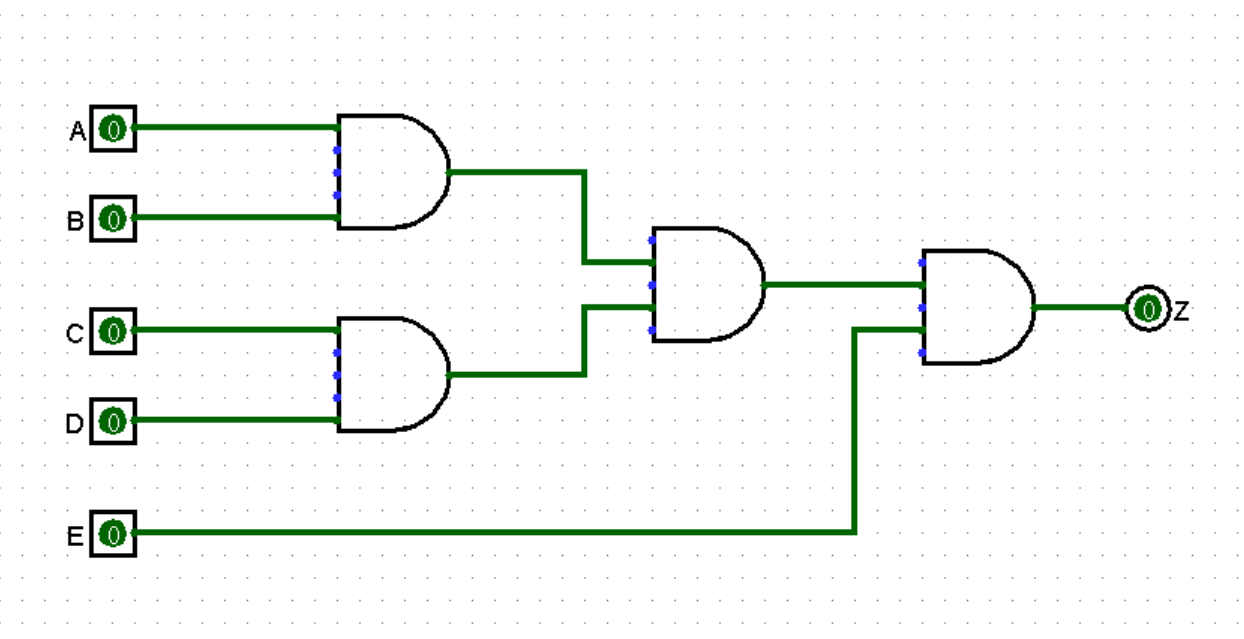
\includegraphics[scale=0.5]{picture/T82.png}
        \end{figure*}
    \end{enumerate}
\section*{T9}
    \begin{enumerate}
        \item [(1)]50个周期后为 1	1	1	0	0	0.
        \item [(2)]至少需要6个周期.
    \end{enumerate}
\section*{T10}
    记$p\ $NAND$\ q=p*q$.
    \begin{enumerate}
        \item [(1)]NOT
        \[  \thicksim p = p*p.   \]
        \item [(2)]AND
        \[  p\ \&\ q  =\left(p*q\right)*\left(p*q\right).  \]
        \item [(3)]OR
        \begin{align*}
            p+q &= \thicksim \left[(\thicksim p)\  \& (\thicksim q)\right]\\
            &=\thicksim\left\{ \left[(p*p)*(q*q) \right]*\left[(p*p)*(q*q) \right]\right\}\\
            &=\left\{ \left[(p*p)*(q*q) \right]*\left[(p*p)*(q*q) \right]\right\}*\left\{ \left[(p*p)*(q*q) \right]*\left[(p*p)*(q*q) \right]\right\}.
        \end{align*}
    \end{enumerate}
\section*{T11}
\begin{enumerate}
    \item [(a)]如图
    \begin{figure*}[htbp]
        \centering
        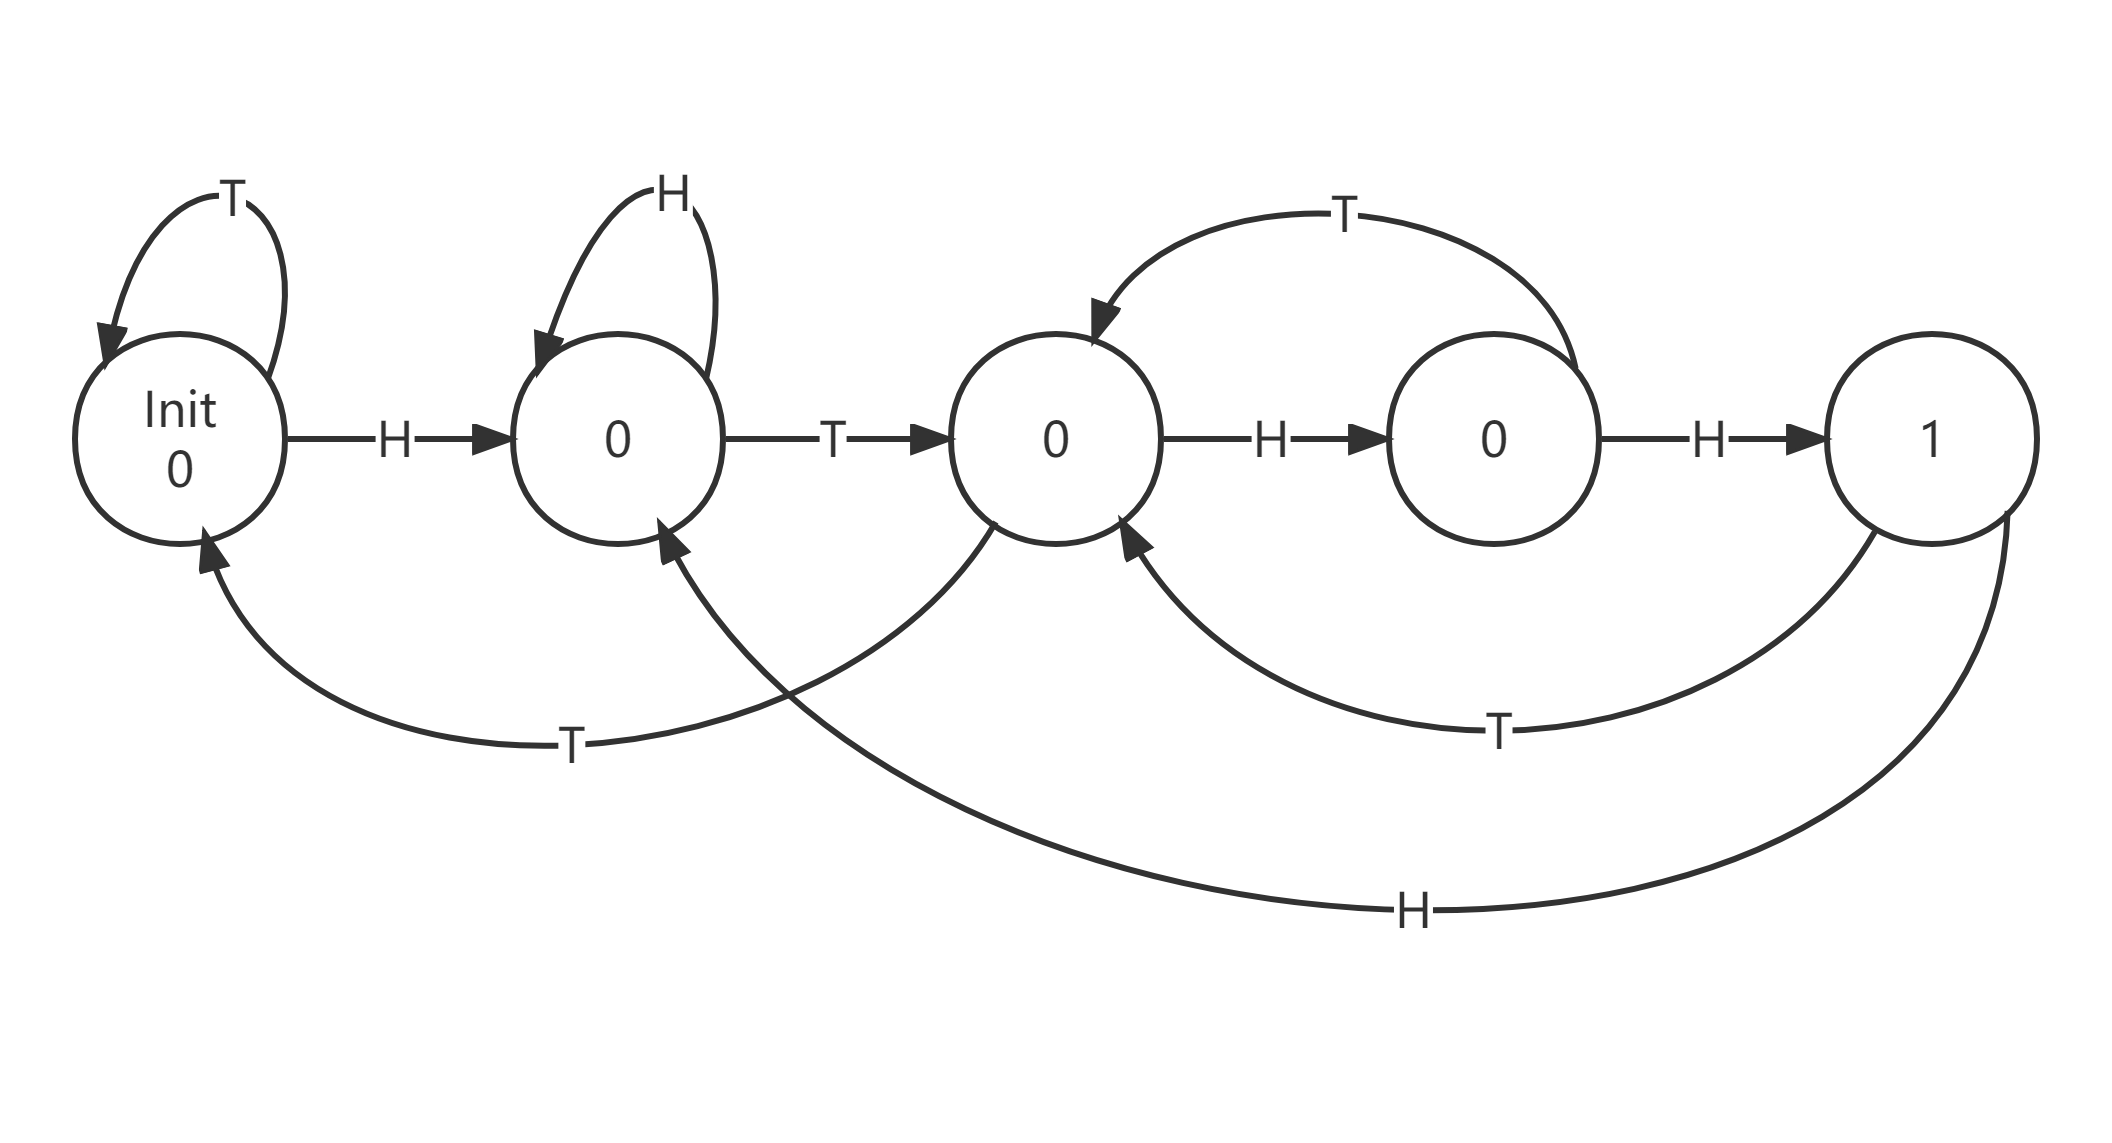
\includegraphics[scale=0.15]{picture/t11.png}
    \end{figure*}
    \item [(b)]需要3个状态变量。
\end{enumerate}

\section*{T12}
\begin{figure*}[htbp]
    \centering
    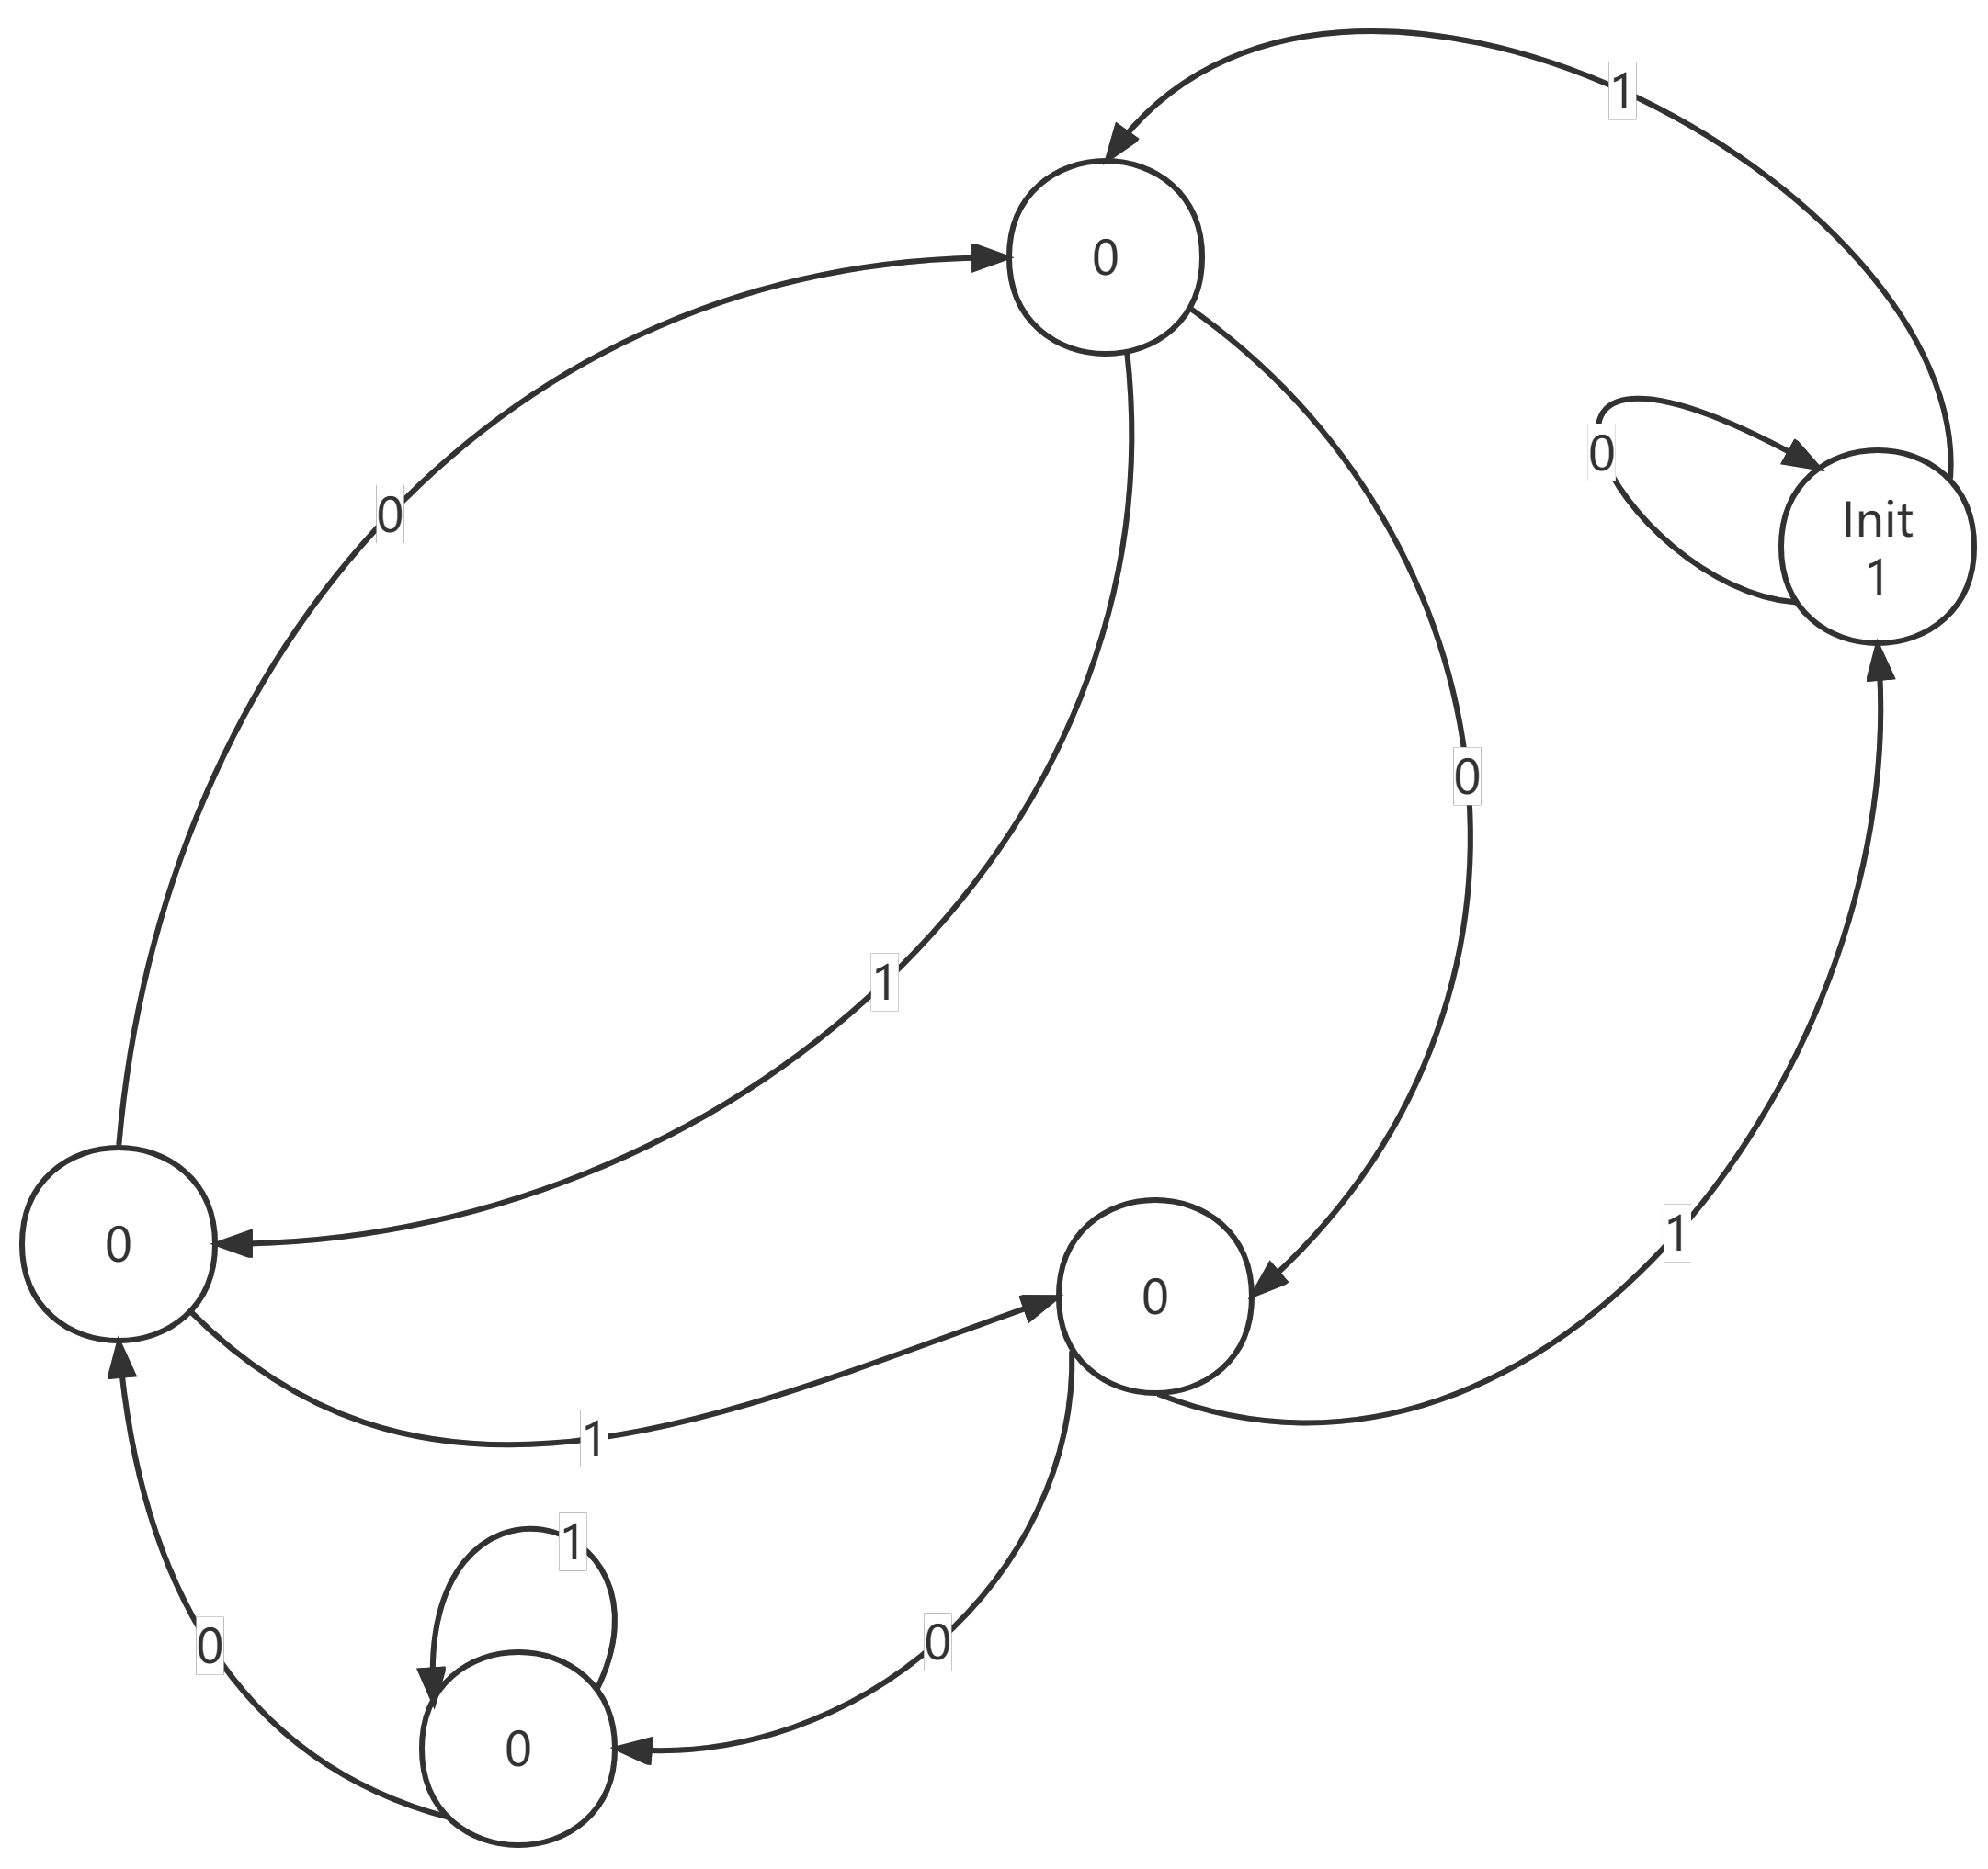
\includegraphics[scale=0.15]{picture/T12.png}
\end{figure*}

\section*{T13}
\[
    8\ bytes\times 2^{8}=2^{6}bits \times 2^{8}= 2^{14}bits =16kb.
\]

\end{document}
 